\documentclass{article}
\usepackage[margin=1in]{geometry}
\usepackage{amsmath,amsthm,amssymb}
\usepackage{bbm,enumerate,mathtools}
\usepackage{tikz,pgfplots}
\usepackage{chessboard}
\usepackage[hidelinks]{hyperref}
\usepackage{multicol} % Problem 35

\newenvironment{question}{\begin{trivlist}\item[\textbf{Question.}]}{\end{trivlist}}
\newenvironment{note}{\begin{trivlist}\item[\textbf{Note.}]}{\end{trivlist}}
\newenvironment{references}{\begin{trivlist}\item[\textbf{References.}]}{\end{trivlist}}
\newenvironment{related}{\begin{trivlist}\item[\textbf{Related.}]\end{trivlist}\begin{enumerate}}{\end{enumerate}}


\begin{document}
  Consider labeled rooted trees where the sum of the labels of the branches
  connected to a vertex is less than the parent label, and the ``top'' label is
  $n$.
  \begin{figure}[!h]
    \centering
    \begin{tikzpicture}
      \node {5}
        child { node {1} }
        child { node {1} }
        child { node {1} }
        child { node {1} };
    \end{tikzpicture}\hspace{0.5cm}
    \begin{tikzpicture}
      \node {5}
        child {
          node {2}
          child { node {1} }
        }
        child { node {1} }
        child { node {1} };
    \end{tikzpicture}\hspace{0.5cm}
    \begin{tikzpicture}
      \node {5}
        child {
          node {2}
          child { node {1} }
        }
        child {
          node {2}
          child { node {1} }
        };
    \end{tikzpicture}\hspace{0.5cm}
    \begin{tikzpicture}
      \node {5}
        child {
          node {3}
          child { node {1} }
          child { node {1} }
        }
        child { node {1} };
    \end{tikzpicture}\\~\\
    \begin{tikzpicture}
      \node {5}
        child {
          node {3}
          child {
            node {2}
            child { node {1} }
          }
        }
        child { node {1} };
    \end{tikzpicture}\hspace{0.5cm}
    \begin{tikzpicture}
      \node {5}
        child {
          node {4}
          child { node {1} }
          child { node {1} }
          child { node {1} }
        };
    \end{tikzpicture}\hspace{0.5cm}
    \begin{tikzpicture}
      \node {5}
        child {
          node {4}
          child {
            node {2}
            child { node {1} }
          }
          child { node {1} }
        };
    \end{tikzpicture}\hspace{0.5cm}
    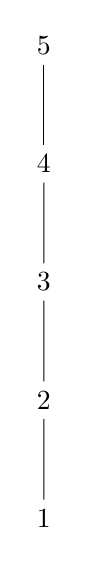
\begin{tikzpicture}
      \node {5}
        child {
          node {4}
          child {
            node {3}
            child {
              node {2}
              child { node {1} }
            }
          }
        };
    \end{tikzpicture}
    \caption{
      Eight examples of trees with a greatest label of $5$:
      $a(5) = a(1)^4 + a(2)a(1)^2 + a(2)^2 + a(3)a(1) + a(4) = 8$
    }
  \end{figure}

\begin{question}
  How many such labels exist?
\end{question}
\begin{related}
  \item What if the same label cannot appear multiple times in the same row?
  \item What if labels are strictly greater than $1$ and the \textit{product} of
    the branches is less than their parent?
\end{related}
\begin{references}
  \item A196545
\end{references}

\end{document}
